\setcounter{chapter}{3}

\chapter{导数与不定积分}

导数刻画了函数关于自变量的变化率,在现实问题中有很多对应的实例,例如:速度、密度、压强、出生率、
死亡率、曲线斜率,等等。导数的引入,极大增强了用数学工具刻画现实问题的能力,可以说其作用是飞跃式的。

不定积分是求导的逆向运算,在Newton、Leibniz揭示了微分和积分的关系后,其重要性才得到了真正的
认识。不定积分的计算是整个微积分学中的一大难点。

\section{导数的概念}

\subsection{函数在一点处的导数}

{\bf 定义4.1.1:}函数$y=f(x)$在$x_0$的某领域内有定义,若
$$\limdx\df{f(x_0+\dx)-f(x_0)}{\dx}$$
存在, 则称{$f(x)$在$x_0$处可导},该极限称为{\it $f(x)$在$x_0$处的导数}, 记为
$${\b f\,'(x_0),\quad \left.\df{\d y}{\d x}\right|_{x=x_0},\quad\left.\df{\d
}{\d x}y\right|_{x=x_0},\quad \left.\df{\d }{\d x}f(x)\right|_{x=x_0}\quad
y'_x|_{x=x_0},\quad \dot{y}(x_0)}$$

{\bf 例:}假设$f\,'(x_0)$存在,则
\begin{enumerate}[(1)]
  \setlength{\itemindent}{1cm}
  \item $\limdx\df{f(x_0-\Delta x)-f(x_0)}{\Delta
  x}=$ \underline{\quad{$-f\,'(x_0)$}\quad} 
  \item $\lim\limits_{h\to 0}\df{f(x_0+2h)-f(x_0)}{h}=$
   \underline{\quad{$2f\,'(x_0)$}\quad} 
  \item $\lim\limits_{h\to 0}\df{f(x_0+h)-f(x_0-h)}{h}=$ 
  \underline{\quad{$2f\,'(x_0)$}\quad}
\end{enumerate}

{\bf 思考:}以上哪个极限存在,与$f(x)$在$x_0$可导等价?

答:只有(3)与可导的定义不等价,因为其中没有提到$f(x_0)$,换言之,{\b 即便$f(x_0)$
没有定义,(3)也可能成立,但这样一来导数的定义就没有意义了!}

\subsubsection{【导数的物理/几何意义】}

\begin{itemize}
  \setlength{\itemindent}{1cm}
  \item {\it 切线斜率:}
  $$k(x_0)=\lim\limits_{x\to x_0}\df{f(x)-f(x_0)}{x-x_0}$$
  \item {\it 瞬时速度:}
  $$v(t_0)=\lim\limits_{t\to t_0}\df{S(t)-S(t_0)}{t-t_0}$$
  \item {\it 出生率:}
  $$\gamma(s_0)=\lim\limits_{s\to s_0}\df{[s_0,s]\mbox{内出生的人口总数}}{s-s_0}$$
\end{itemize}

{\bf 导数:函数关于自变量的变化率!}\ps{当自变量发生变化时,函数值发生的相应变化与之的比率}

{\bf 例:}已知函数$f(x)$在点$x_0$处可导,求曲线$y=f(x)$在该点的切线和法线方程。

\begin{itemize}
  \setlength{\itemindent}{1cm}
  \item {\it\b 切线:\quad $y=f(x_0)+f'(x_0)(x-x_0)$}
  \item {\it\b 法线:\quad $y=f(x_0)-\df1{f'(x_0)}(x-x_0)\quad(f'(x_0)\ne 0)$}
\end{itemize}

{\bf 例:}若抛物线$y=x^2$上有三个不同号点处的法线交于一点,这三个点的横坐标需要满足什么条件?

[提示]: 设三个点的横坐标分别是$a_1,a_2,a_3$。

情形一:若某个$a_i=0$(不妨为$a_1=0$),显然由对称性可知,必有$a_2=-a_3$。

情形二:若$a_1,a_2,a_3$均非零,我们可以给出$a_i(i=1,2,3)$处的法线方程
$$y=a_i^2-\df1{2a_i}(x-a_i)$$
化简后可得
$$\df{a_1+a_2}{a_3}=\df{a_1+a_3}{a_2}=\df{a_2+a_3}{a_1}$$
进而
$$\df{a_1+a_2+a_3}{a_3}=\df{a_1+a_2+a_3}{a_2}=\df{a_1+a_2+a_3}{a_1}$$
显然$a_,a_2,a_3$相互不同,故必有$a_1+a_2+a_3=0$。

{\b {\bf 思考:}可导等价于有切线吗?({\it 否,若切线是铅直方向的,则导数没有意义!})}

{\bf 例:}讨论函数$f(x)=\sqrt[3]x$在点$x=0$是否可导?

\subsubsection{【导数存在的条件】}

{\bf 定理4.1.1:}$f(x)$在$x_0$可导,当且仅当在该点的左、右导数存在且相等。
\ps{\b 左导数:$f'_-(x_0)$\\ 右导数$f'_+(x_0)$,注意和导函数的左右极限的区别}

{\bf 定理:}初等函数在其定义域内是处处可导的。\ps{而且其任意阶导函数也是可导的!}

{\bf 定理4.1.2:}$f(x)$在一点可导,则一定在该点连续。

{\bf 例:}函数$f(x)=x^2D(x)$在$x=0$可导,但在其他地方都不连续。

{\bf 教材-例8:}确定常数$a,b$的值,使得函数
$$f(x)=\left\{\begin{array}{ll}ax+b,& x>0\\
e^x,& x\leq 0\end{array}\right.$$
在$x=0$可导。

{\bf 例:}确定$a$的值,使$y=ax^2$与$y=\ln x$相切。

{\bf 例:}设$f(x)=\left\{\begin{array}{ll}
\df{1-\sqrt{1-x}}{x}, & x<0,\\
a+bx, & x\geq 0
\end{array}\right.$,求$a,b$使$f(x)$处处可导。\ps{导数计算过于复杂}

{\bf 例:}已知$f(x)=\left\{\begin{array}{ll}
\sin x,& x<0\\ x,& x\geq 0
\end{array}\right.$
求$f'(x)$

{\bf 例:}问题讨论
\begin{enumerate} 
  \setlength{\itemindent}{1cm}
  \item 若$f(x),g(x)$在$x_0$均不可导,是否$f(x)+g(x),$ $f(x)g(x)$必不可导?
  ({$\times$}) 
  \item 若对任意$x\in (a,b)$,恒有$f(x)<g(x)$,且$f(x),g(x)$均在$(a,b)$内
  可导,问是否必有$f\,'(x)<g'(x)$? ({$\times$}) 
  \item $f(x)$可导,则$|f(x)|$可导?反之呢?({$\times$})
  \item 若$f(x)$在$\mathbb{R}$上可导,且$\limx{+\infty}f(x)=\infty$,是否
  必有$\limx{+\infty}f\,'(x)=\infty$?反之呢? ({$\times$})
  \item 若$f(x)$在$(a,b)$内可导,且$\limx{a^+}f(x)=\infty$,是否
  必有$\limx{a^+}f\,'(x)=\infty$? 反之呢?({$\times$}) 
  \item 若$f(x)$可导且为奇(偶)函数,则$f\,'(x)$也有奇偶性? 
  (相应的$f'(0)$有什么特点?偶函数,$f'(0)=0$)({$\surd$}) 
  \item 若$f(x)$可导且为周期函数,则$f\,'(x)$也是周期函数? ({$\surd$})
\end{enumerate}

{\bf 例:}设$f(x)=\sum\limits_{i=1}^na_i\sin
ix$,其中$a_i(i=1,2,\ldots,n)$为常数,且对任意$x\in\mathbb{R}$, 
$|f(x)|\leq |\sin x|$,证明:
$$\left|a_1+2a_2+\ldots+na_n\right|\leq 1$$

[提示]:$f(0)=0$,于是
$$|f'(0)|=\limx{0}\df{|f(x)|}{|x|}\leq\limx{0}\df{|\sin x|}{|x|}=1$$
事实上$f'(0)=a_1+2a_2+\ldots+na_n$.

{\bf 思考:}
\begin{enumerate} 
  \setlength{\itemindent}{1cm}
  \item $f'(x_0)$和$[f(x_0)]'$,$f'(x)$和$[f(x)]'$有何异同?
  \item $f'_+(x_0)$和$f'(x_0+0)$有何区别?\ps{有些书上也把$f'(x_0+0)$记为$f'(x_0^+)$}
  \item $f(x)=g(x)\Rightarrow f'(x)=g'(x)$?反之呢?
  \item 园面积$S(r)$关于直径的导数$S'(r)=l(r)$为圆周长,
  球体积关于直径的导数为表面积,如何解释?类似的,(定长)圆柱体的体积关于截面半径的导数
  等于其与侧面积?矩形的体积关于各边长的导数等于其对应的截面积?
\end{enumerate}

\subsection{导函数}

{\bf 例}({\it 一些常用函数的导函数})\ps{利用定义验证以下的导函数是复习函数极限计算的好方法!}
\begin{enumerate}[(1)]
  \setlength{\itemindent}{1cm}
  \item $f(x)=C\;(C\mbox{为常数})$ \hfill $f\,'(x)=0$ 
  \item $f(x)=x^n\;(n\in\mathbb{Z})$ \hfill $f\,'(x)=nx^{n-1}\,(n\ne
  0)$ 
  \item $f(x)=e^x$ \hfill $f\,'(x)=e^x$ 
  \item $f(x)=\ln|x|$ \hfill $f\,'(x)=\df 1x$ 
  \item $f(x)=\sin x$ \hfill $f\,'(x)=\cos x=\sin\left(x+\df{\pi}2\right)$ 
  \item $f(x)=\cos x$ \hfill $f\,'(x)=-\sin x=\cos\left(x+\df{\pi}2\right)$
\end{enumerate}

\section{导数的计算}

\subsection{四则运算的求导法则}

{\bf 定理4.2.1:}设$u(x),v(x)$均在$x$可导,则
\begin{enumerate}[(1)]
  \setlength{\itemindent}{1cm}
  \item $[u(x)\pm v(x)]'=u'(x)\pm v'(x)$ 
  \item $[u(x)v(x)]' =u'(x)v(x)+u(x)v'(x)$ \ps{自行推导$(uvx)'$的公式}
  \item $\left[\df{u(x)}{v(x)}\right]'
  =\df{u'(x)v(x)-u(x)v'(x)}{v^2(x)}\;(v(x)\ne 0)$
\end{enumerate}

{\bf 教材-例2-4:}计算以下函数的导函数
\begin{enumerate}[(1)]
  \setlength{\itemindent}{1cm}
  \item $f(x)=2x^3+3x-4x+5-\df 6x$ 
  \item $f(x)=e^x\sin x$ 
  \item $f(x)=\df{x-1}{x+1}$ 
  \item $f(x)=\df 1{\ln x}$ 
  \item $f(x)=\tan x$ \hfill $f\,'(x)=\sec^2 x$ 
  \item $f(x)=\sec x$ \hfill $f\,'(x)=\sec x\tan x$
\end{enumerate}

{\bf 例:}已知$f(x)$可导,且无零点,证明:$y=f(x)$和$y=f(x)\sin x$
在相交的位置必相切。

{\bf 思考:}函数$y=f(x)$和$y=f(x)\sin x$的图像有何关系?

\begin{center}
	\resizebox{!}{4cm}{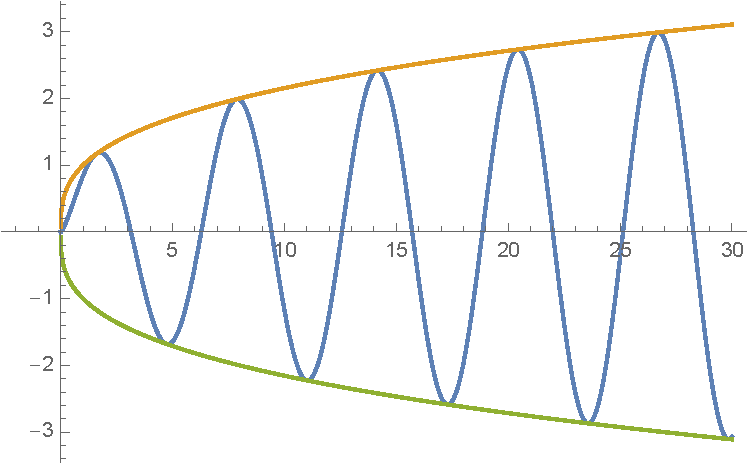
\includegraphics{./images/ch4/x3Sinx.pdf}}\quad
	\resizebox{!}{4cm}{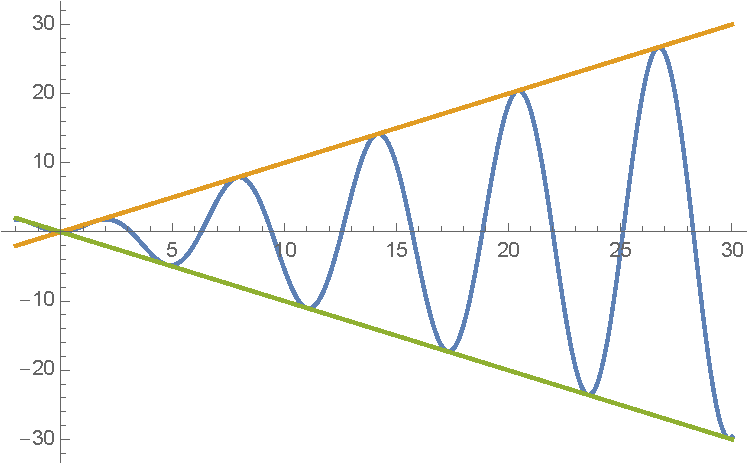
\includegraphics{./images/ch4/xSinx.pdf}}
	
	$y=x^{1/3}\sin x$\hspace{5cm}$y=x\sin x$
	
	\resizebox{!}{4cm}{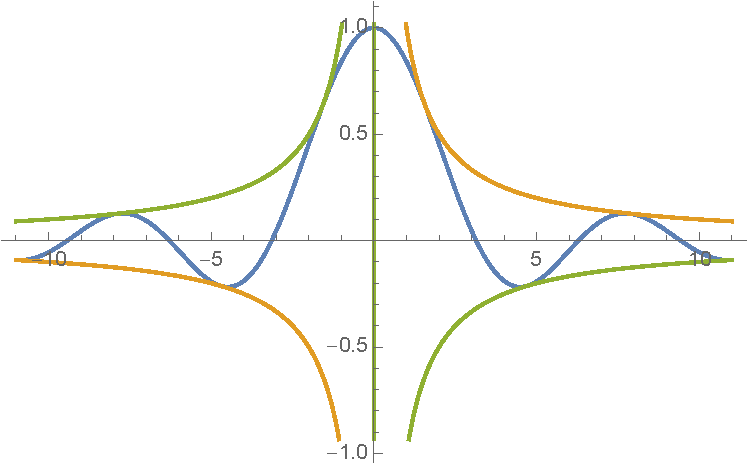
\includegraphics{./images/ch4/1xSinx.pdf}}\quad
	\resizebox{!}{4cm}{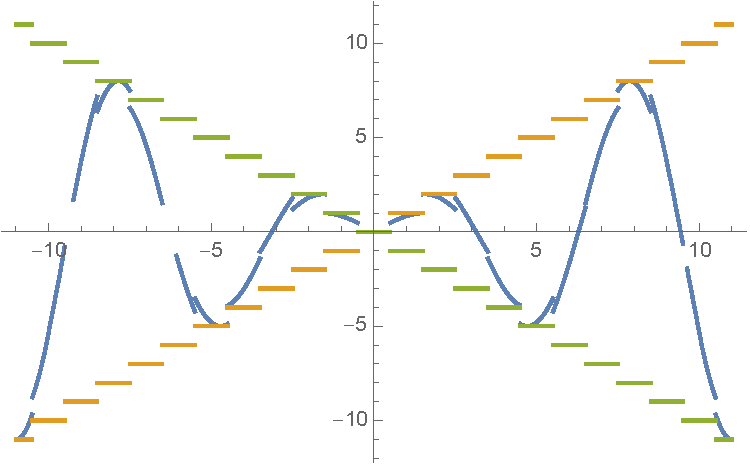
\includegraphics{./images/ch4/rxSinx.pdf}}
	
	$y=\df1x\sin x$\hspace{5cm}$y=[x]\sin x$
	
	\resizebox{!}{4cm}{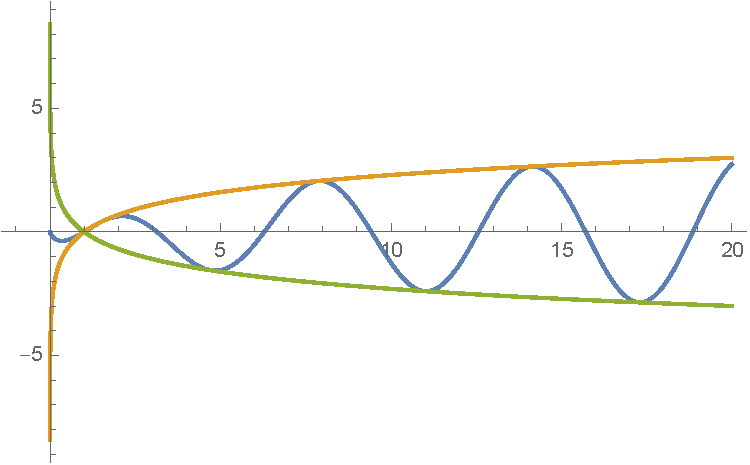
\includegraphics{./images/ch4/lnxSinx.pdf}}\quad
	\resizebox{!}{4cm}{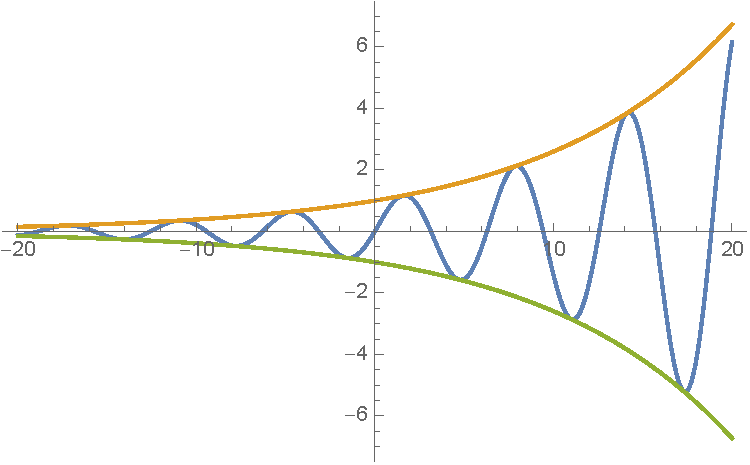
\includegraphics{./images/ch4/11xSinx.pdf}}
	
	$y=\ln x\sin x$\hspace{5cm}$y=1.1^x\sin x$
\end{center}

\subsection{反函数求导法则}

{\bf 定理4.2.2:}设$y=f(x)$是$x=\varphi(y)$的反函数,
若$x=\varphi(y)$在$y$处可导,且$\varphi'(x)\ne 0$,则
$y=f(x)$在点$x=\varphi(y)$处可导,且\ps{\b 正确理解和使用下面这个公式是本节的难点!}
$${\b f\,'(x)=\df{1}{\varphi'(y)}}$$

{\bf 例:}考虑函数$y=e^x$,我们已知$(e^x)'_{\b x}=e^x$,故
$$(\ln y)'_{\b y}=\df1{(e^x)'_{\b x}}=\df1{e^x}=\df1y$$

{\bf 例7-8:}计算下列函数的导函数
\begin{enumerate}[(1)]
  \setlength{\itemindent}{1cm}
  \item $f(x)=\arcsin x$ \hfill $f\,'(x)=\df{1}{\sqrt{1-x^2}}$ 
  \item $f(x)=\arctan x$ \hfill $f\,'(x)=\df{1}{1+x^2}$
\end{enumerate}

{\bf 例:}设$f(x)=x^5+2x^3+4x,(-\infty<x<+\infty)$
\begin{enumerate}[(1)]
  \setlength{\itemindent}{1cm}
  \item 证明$f$可逆;
  \item 设$g=f^{-1}$,计算$g(7)$
  \item 计算$g'(7)$
\end{enumerate}

\subsection{复合函数的求导法则}

{\bf 定理4.2.3}({\it 链式法则})设函数$u=\varphi(x)$在$x$处可导,
函数$y=f(u)$在$u=\varphi(x)$处可导,则复合函数$y=f[\varphi(x)]$
在$x$处可导,且
$${\b y'_x=f_u'(u)\varphi_x'(x)}$$

{\bf 教材-例5:}计算下列函数的导函数
\begin{enumerate}[(1)]
  \setlength{\itemindent}{1cm}
  \item $y=a^x\;(a>0,a\ne 1)$ \hfill $y'=a^x\ln a$ 
  \item $y=x^a$ \hfill $y'=ax^{a-1}$
\end{enumerate}

{\bf 例:}若$f$可导,且$[f(x^2)]'=[f^2(x)]'$,则$f(1)=1$或$f'(1)=0$.

{\bf 教材-例10-19:}计算下列函数的导函数
\begin{enumerate}[(1)]
  \setlength{\itemindent}{1cm}
  \item $y=e^{x^2}$ 
  \item $y=\sin (3x+2)$ 
  \item $y=\cos^2(1-2x)$ 
  \item $y=\ln\sin e^{-x}$ 
  \item $y=(1-30x)^{50}$ 
  \item $y=\ln(1+x^2)$ 
  \item $y=e^{\sqrt{1-3x}}$ 
  \item $y=x^x$ 
  \item $y=e^{\tan\frac 1x}$
\end{enumerate}

{\b{\bf 例:}形如$y=u^v$的函数求导,其中$u,v$均可导\ps{难点!注意这类函数并不属于基本的初等函数}
\begin{enumerate}[(1)]
  \setlength{\itemindent}{1cm}
  \item $y=x^x$
  $$(x^x)'=(e^{x\ln x})'=e^{x\ln x}\left(\ln x+x\cdot\df1x\right)=x^x(1+\ln x)$$
  \item $y=x^{x^x}$
  \item $y=\left(x^x\right)^x$
\end{enumerate}
}

{\bf 教材-例20:}设$f(x)$可导,且$f\,'\left(\df{\pi}{4}\right)=1$,求
$$\varphi(x)=f\left(\arctan\df{1+x}{1-x}\right)$$
在$x=0$处的导数。

\subsection{高阶导数}

{\bf 定义4.2.1}({\it $n$阶导数})
$$f^{\,(n)}(x)=\df{\d^nf(x)}{\d x^n}=\left[f^{\,(n-1)}(x)\right]'_x$$

{\bf 教材-例34:}求函数$f(x)=x^3+2x^2-3x+10$的各阶导函数。

{\bf 注:}若$P(x)$为$n$次多项式,则$P^{(n+1)}(x)=0$。

{\bf 教材-例25-26:}求以下函数的$n$阶导数
\begin{enumerate}[(1)]
  \setlength{\itemindent}{1cm}
  \item $y=\df 1x$ \hfill $y^{(n)}(x)=(-1)^n\df{n!}{x^{n+1}}$ 
  \item $y=\sin x$ \hfill
  $y^{(n)}(x)=\sin\left(\df{n\pi}{2}+x\right)$ 
  \item $y=xe^x$ \hfill $y^{(n)}(x)=(n+x)e^x$
  \item $y=e^{ax}\sin bx$

[提示]:
$$y'=e^{ax}(a\sin bx+b\cos
bx)=\sqrt{a^2+b^2}e^{ax}\sin(bx+\varphi),
\;\tan\varphi=\df ba$$
$$y^{(n)}=\left(a^2+b^2\right)^{n/2}e^{ax}\sin(bx+n\varphi)$$ 
\end{enumerate}

{\bf 【Leibnitz公式】}\ps{\b 难点+考点!}

$${\b{\left[u(x)v(x)\right]^{(n)}=
\sum\limits_{k=0}^nC_n^ku^{(n-k)}(x)v^{(k)}(x)}}$$

{\bf 教材-例27:}设$y=x^3e^x$,求$y^{(10)}$。

{\bf 例:}$(x^2\sin x)^{(80)}=(x^2-6320)\sin x-160x\cos x$。

{\bf 例:}
$$\left(\df{2x}{1-x^2}\right)^{(n)}=n!\left[\df1{(1-x)^{n+1}}
-\df{(-1)^n}{(1+x)^{n+1}}\right]$$

{\bf 例:}设$y=\arctan x$,求$y^{(n)}(0)$

[提示]:
$$y'=\df1{1+x^2}\quad \Rightarrow\quad (1+x^2)y'=1,$$
利用Leibniz公式可得
$${\b (1+x^2)y^{(n)}+2nxy^{(n-1)}+n(n-1)y^{(n-2)}=0,}$$
令$x=0$,可得
$$y^{(n)}(0)+n(n-1)y^{(n-2)}(0)=0\quad
\Rightarrow\quad y^{(n)}(0)=-n(n-1)y^{(n-2)}(0)$$
注意到$y'(0)=1,y''(0)=0$,故
$$y^{(n)}(0)=\left\{\begin{array}{ll}
0,\quad& n=2k\\
(-1)^k(2k+1)!,\quad& n=2k+1
\end{array}\right.$$

\begin{shaded}
[提示]:非典型的解法
$$y'=\df1{1+x^2}=\cos^2y=\cos y\sin\left(y+\df{\pi}2\right)$$
$$y''=\cos^2y\cos\left(2y+\df{\pi}2\right)=\cos^2y\sin2\left(y+\df{\pi}2\right)$$
$$y'''=2\cos^3y\sin3\left(y+\df{\pi}2\right)$$
$$y^{(n)}=(n-1)!\cos^ny\sin n\left(y+\df{\pi}2\right)$$
记$z=\arctan\df1x=\df{\pi}2-y$
$$y^{(n)}=(n-1)!\df1{(1+x^2)^{n/2}}\sin n(\pi-z)=
(n-1)!\df1{(1+x^2)^{n/2}}\sin n\arctan\df1x$$
\end{shaded}
{\bf 习题集P77-例23:}设$y=(\arcsin x)^2$,求$y^{(n)}(0)$

\subsection{隐函数求导法则}

{\bf 隐函数:}由形如$f(x,y)=0$的方程所确定的函数

问题:由隐函数方程$f(x,y)=0$解出变量$y$关于$x$的导数

解法:{\it\b 视$y$为$x$的函数$y(x)$,则原方程即为
$$f(x,y(x))=0,$$
两边同时关于$x$求导,然后利用求导后的方程解出$y'_x$即可
}

{\bf 教材-例28:}设$y=y(x)$是由方程
$$x^3+y^3=3xy$$
所确定的隐函数,满足$y(3/2)=3/2$,求其
在点$(3/2,3/2)$处的切线方程。

{\bf 解}:将$y$视为$x$的函数,对已知方程两边关于$x$求导,可得
\ps{\b 在隐函数方程求导的结果中,允许同时包含$x$和$y$}
$$3x^2+3y^2y'=3y+3xy'\quad\Rightarrow\quad
y'=\df{x^2-y}{x-y^2},$$
带入$(x,y)=(3/2,3/2)$可得$y'(3/2)=-1$,故所求切线方程为
$$y=-x+3.$$

\begin{center}
	\resizebox{!}{5cm}{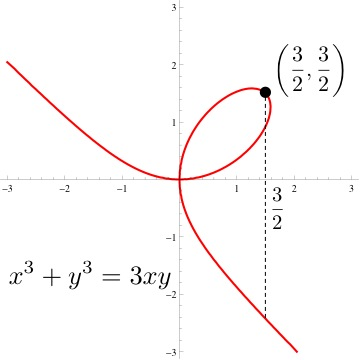
\includegraphics{./images/ch4/x3y33xy.jpg}}
\end{center}

{\bf 教材-例29:}设$y=y(x)$是由方程$y^2=x^2-\cos y$所确定的隐函数,求$y''(x)$。

\begin{center}
	\resizebox{!}{6cm}{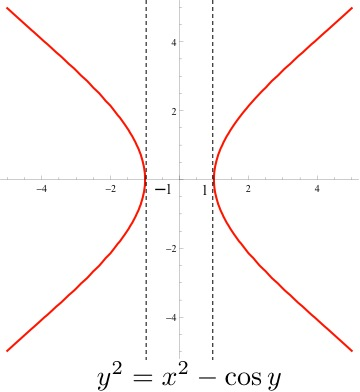
\includegraphics{./images/ch4/y2x2-cosy.jpg}}
\end{center}

{\bf 教材-例30:}求函数$y=(x^2+1)\sqrt[3]{(x-2)^2(x^2+x)}$的导数。

{\bf 例:}设$x^2+xy+y^2=1$,则
$$y'=-\df{2x+y}{x+2y},\quad y''=-\df6{(x+2y)^3}$$
$$y'''=-\df{54x}{(x+2y)^5}$$
$x+2y=0$恰好与经过角度旋转(逆时针$\pi/6$)的椭圆的交点出切线与$y$轴平行。

\begin{shaded}
	{\bf 例:}证明椭圆上任一点处的法线平分该点与两个焦点的连线所夹角。

	[提示]:{\it 如图
	\begin{center}
		\resizebox{!}{5cm}{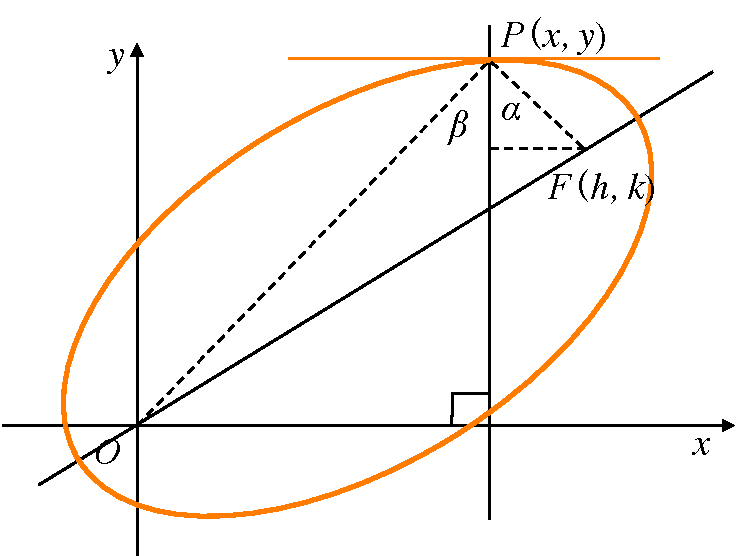
\includegraphics{./images/ch4/rollEc.pdf}}
	\end{center}
	只需证明上半椭圆上任一点有此性质即可。通过旋转椭圆,总可以是点$P(x,y)$处的切线为水平的,
	即$y'(x)=0$。
	此时,设椭圆的两个焦点分别为$(0,0)$和$(h,k)$,则由椭圆的几何性质,有
	$$\sqrt{x^2+y^2}+\sqrt{(x-h)^2+(y-k)^2}=L,$$
	其中$L$为某个确定的值。两端同时对$x$求导,并带入$y'(x)=0$,可得
	$$\df{x}{\sqrt{x^2+y^2}}=\df{h-x}{\sqrt{(x-h)^2+(y-k)^2}}.$$
	由图上不难看出该式也即$\sin\alpha=\sin\beta$,即证。}
		
[又解]:
设椭圆为$\frac{x^2}{a^2}+\frac{y^2}{b^2}=1$,左右焦点分别为$F_1,F_2$,椭圆上任意一点$P(x_0,y_0)$。
$P$点处法线平分$\angle F_1PF_2$的充分必要条件为$P$点处切线平分$\angle F_1PF_2$的外角。
$\frac{x^2}{a^2}+\frac{y^2}{b^2}=1$两边同时关于$x$求导,有
$$\frac{2x}{a^2}+\frac{2yy’}{b^2}=0,$$
得
$$y’=-\frac{b^2x}{a^2y}$$
所以$P$处的切线斜率$k=-\frac{b^2x_0}{a^2y_0}$。
又$\angle 1,\angle 2\in(0,\pi/2)$,且
$$\tan\angle 1=-\frac{b^2y_0}{a^2y_0}-\frac{y_0}{x_0}-c=\frac{b^2}{cy_0},$$
同理$\tan\angle 2= \frac{b^2}{cy_0}$,
故$\angle 1=\angle 2$。

\end{shaded}

\subsection{参数方程求导法则}

设函数$y=y(x)$由参数方程
$$\left\{
\begin{array}{l}
x=\varphi(t)\\
y=\psi(t)
\end{array}
\right.$$
确定, $x=\varphi(t)$可逆, 则\ps{\b 要求熟练掌握有关的推导,难点!}
$${\b y'(x)=\df{\psi'(t)}{\varphi'(t)}}$$

$${\b y''(x)=\df{\psi''(t)\varphi'(t)-\psi'(t)\varphi''(t)}{[\varphi'(t)]^3}}$$

{\bf 教材-例31:}求抛物线$x=y^2$在$(1,1)$和$(4,-2)$处的切线方程。

{\bf 教材-例32:}已知$\left\{\begin{array}{l}x=t-\sin t\\
y=1-\cos t\end{array}\right.$,求$y''(x)$。

\begin{center}
	\resizebox{!}{3cm}{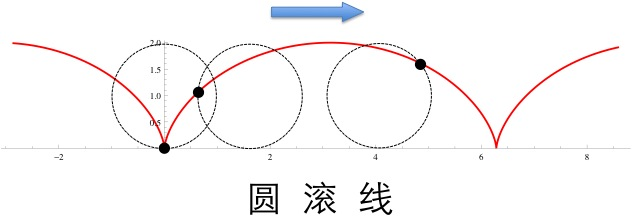
\includegraphics{./images/ch4/sphereRoll.jpg}}
\end{center}

{\bf 例:}设$\left\{\begin{array}{l}x=f\,'(t)\\ y=tf\,'(t)-f(t)
\end{array}\right.$,求$\df{\d^2y}{\d x^2}$,其中$f\,''(x)$存在且不为零。

{\bf 例:}$x^2+xy+y^2=1$的参数方程
$$x=\df2{\sqrt3}\cos t,\quad y=\sin t-\df1{\sqrt3}\cos t$$
$$y'_x=-\df{\sqrt3}2\cot t-\df12$$
$$y''_{xx}=-\df34\csc^3t$$
$$y'''_{xxx}=-\df{9\sqrt3}8\df{\cos t}{\sin^5t}$$
事实上,$t=\arccos\df{\sqrt3}2x$,当$\sin t\ne0$,也即$t\ne2k\pi-\df{\pi}6$
时以上导数才有意义。

{\bf 例:}Archimedes螺线$\rho=a\theta$与双曲螺线$\rho=a/\theta$相交处相互垂直。

\begin{center}
	\resizebox{!}{8cm}{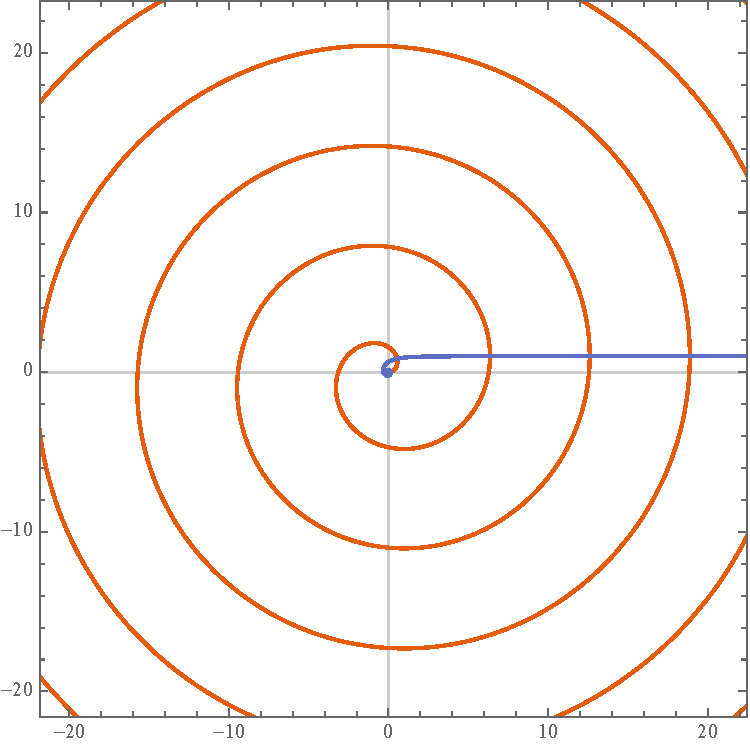
\includegraphics{./images/ch4/arCurve.pdf}}
	
	{\it$\rho=\theta$和$\rho=1/\theta$\quad($\theta\in(0,10\pi)$)
	
	两曲线的交点为$\theta(k)=-k\pi+\sqrt{k^2\pi^2+1},(k\in\mathbb{N})$
	
	但是注意到只有当$k=0$时,曲线交点处的$\theta$值才对两个函数来说才是相同的,
	
	因此,两条曲线真正意义上的交点只有$\theta=1$
	}
\end{center}

[提示]:两曲线的参数方程分别为
$$
\left\{\begin{array}{l}
	x=a\theta\cos\theta\\
	y=a\theta\sin\theta
\end{array}\right.
\quad\quad\quad
\left\{\begin{array}{l}
	x=\df{a}{\theta}\cos\theta\\
	y=\df{a}{\theta}\sin\theta
\end{array}\right.
$$
相应的曲线斜率分别为
$$y'_x=\df{\sin\theta+\theta\cos\theta}{\cos\theta-\theta\sin\theta}
\quad\quad\quad
y'_x=-\df{\theta\cos\theta-\sin\theta}{\theta\sin\theta+\cos\theta}
$$
显然$\theta=1$时二者的乘积为$-1$,这意味着两条曲线在交点处垂直!
\ps{$k\ne0$时,从图像上看两条曲线也是相互垂直的,如何证明呢?}

\section{微分}

\subsection{概念}

{\bf 【局部线性化和“以直代曲”】}

若$f(x)$在$x_0$可导,则
$$f(x)=f(x_0)+f\,'(x_0)(x-x_0)+\circ(x-x_0)\quad(x\to x_0)$$ 
即:{\bf 在$x_0$附近,$f(x)$可以近似地表示为一个线性函数} 
$$f(x)\approx f(x_0)+f\,'(x_0)(x-x_0)$$

\begin{center}
	\resizebox{!}{6cm}{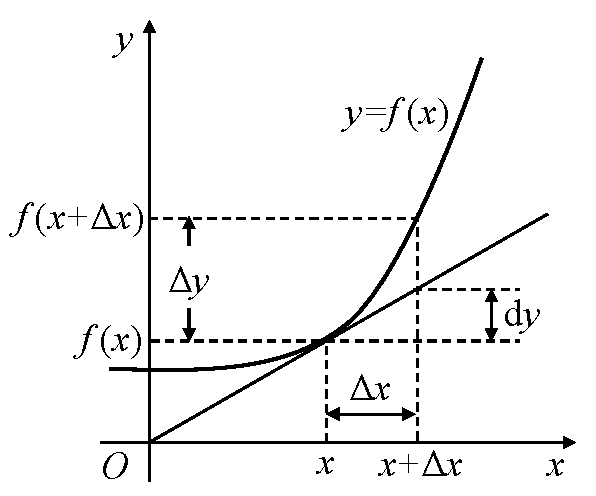
\includegraphics{./images/ch4/dy.pdf}}
\end{center}

{\bf 定义4.3.1:}设$y=f(x)$在$x_0$的某领域内有定义,
若存在与$\Delta x$无关的常数$A$,使得$\Delta y=f(x_0+\Delta x)-f(x_0)$满足
$$\Delta y=A\Delta x+\circ(\Delta x)\;(\Delta x\to 0)$$ 
则称$y=f(x)$在$x_0${\it 可微}, $A\Delta x$称为{\it $y=f(x)$在$x_0$处的微分},
记为 $$\left.\d y\right|_{x=x_0}\quad \mbox{或} \quad
\left.\d f(x)\right|_{x=x_0}$$

{\bf 定理4.3.1:}设$y=f(x)$在$x_0$可微,当且仅当$y=f(x)$在$x_0$可导,且
$$\left.\d y\right|_{x=x_0}=f\,'(x_0)\d x\quad 
\mbox{或} \quad\left.\d f(x)\right|_{x=x_0}=f\,'(x_0)\d x$$

{\bf P196-例3:}设$f(x)=x^3+2x^2-3x+6$,求$\d f(x)$和$\d f(x)|_{x=1}$,
并求其在$(1,6)$处的局部线性化函数$L(x)$。

\subsection{微分的运算法则}

{\bf 定理4.3.2}(四则运算)设$u(x),v(x)$可导,则
\begin{enumerate}[(1)]
  \setlength{\itemindent}{1cm}
  \item $\d (u\pm v)=\d u\pm \d v$
  \item $\d(uv)=v\d u+u\d v$
  \item $\d\df uv=\df{v\d u-u\d v}{v^2}$
\end{enumerate}

{\bf 定理4.3.3}(复合运算)设$y=f(u),u=\varphi(x)$均可微,
则$y=f[\varphi(x)]$可微,
$$\d y=f\,'(u)\d u=f\,'(u)\varphi'(x)\d x$$

{\bf P201-例6:}求函数$y=e^{2x-1}\sin x$的微分。

{\bf P202-例7:}试将下列微分形式表示为某一函数的微分 
\begin{enumerate}[(1)]
  \setlength{\itemindent}{1cm}
  \item $x^2\d x$ 
  \item $e^{2x}\d x$ 
  \item $\cos(5x-1)\d x$ 
  \item $\df{1}{1+2x^2}\d x$
\end{enumerate}

\section{变化率和相关变化率}

{\bf 变化率:}一个变量随另一个变量变化过程中,相对于后者发生变化的速率,或者
{\it 二者的相关变化量的比值}

{\bf 导数:}对于各种变化率的数学抽象

\begin{itemize}
  \setlength{\itemindent}{1cm}
  \item {斜率}:函数值关于自变量的变化率 
  \item {速度}:位移关于时间的变化率 
  \item {密度}:质量关于体积的变化率 
  \item {电流强度}:电量关于时间的变化率 
  \item {边际收益}:收益关于投入的变化率 
  \item {\ldots\ldots} 
\end{itemize}

{\bf P209-例7:}有一深度$8$m,上底直径$8$m的圆锥形容器,
以$4$m$^3$/min的速率向其中注水,当容器中水深$5$m时,水面上升的速度是多少?

{\bf P209-例8:}甲乙两船分别向南和向东航行。在初始时刻,甲船恰位于乙船北方
$40$km处,后来在某一时刻测得甲船向南航行了20km,此时速度为15km/h;
乙船向东航行了15km,此时速度为25km/h。问该时刻两船是在相互靠近还是远离,
二者的相对速度是多少?

{\bf 例:}质点$P$沿抛物线$x=y^2(y>0)$移动。$P$的横坐标$x$的变化速度为$5$cm/s。
当$x=9$cm时,点$P$到原点的距离的变化速率是多少?

{\bf [hint]:}
$$\df{\d}{\d t}\sqrt{x^2+y^2}=\left(\sqrt{x^2+x}\right)'_xx'_t
=\df{5(2x+1)}{\sqrt{x^2+x}}$$
代入$x=9$,可得其值为$\df{95}{6\sqrt10}$(cm/s)

{\bf 例:}钟表的时针和分针长度分别为$a$(cm)和$b$(cm),求$12:20$分,两针端点分离的速率。

{\bf [hint]:}两针的夹角变化速率$\theta'_t=\df{\pi}{30}-\df{\pi}{360}
=\df{11}{360}\pi$(弧度/分钟)。12:20时,$\theta=\df23\pi-\df{\pi}{18}
=\df{11}{18}\pi$。利用余弦定理
$$s^2=a^2+b^2-2ab\cos\theta$$
答案$0.38$(cm/min)

{\bf 例:}圆形广场中央立着高度为$h$的灯柱,灯$A$位于灯柱顶端。
广场上任一点$P$处的照明强度$I$与该点到灯的距离的平方成反比,与光线与灯柱的
夹角的余弦成正比。一个人从距离灯柱$x$m处以速度$v$m/s沿径向离开柱子,求
其脚部的光照强度关于时间的变化率。

{\bf [hint]:}由已知
$$I=k\df{h}{(x^2+h^2)^{\frac32}}.$$
从而
$$I'_t=I'_xx'_t=vI'_x=-\df{xvkh}{(x^2+h^2)^{\frac52}}$$

{\bf 例:}一个长度为$l$的杆,一段连接半径为$r$的转轮,一段位于$x$轴上。转轮的中心
位于原点,以每分钟$m$转的速度逆时针旋转,求:杆位于$x$轴上的一端的运动速率。

{\bf [hint]:}如图
\begin{center}
	\resizebox{!}{4cm}{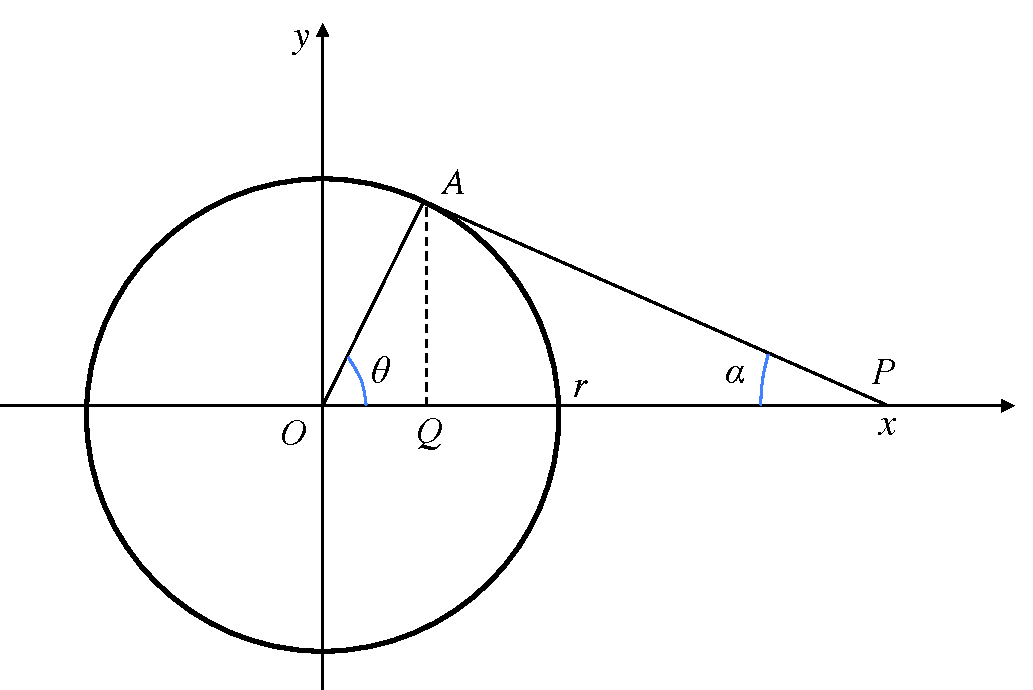
\includegraphics{./images/ch4/rollbar.pdf}}
\end{center}
$$\sin\theta=\df{|AQ|}r,\quad \sin\alpha=\df{|AQ|}{l}$$
从而$\sin\alpha=\df rl\sin\theta$,进而$\alpha=\arcsin\left(
\df rl\sin\theta\right)$。
$$x=r\cos\theta+l\cos\alpha=r\cos\theta+l\cos
\left[\arcsin\left(\df rl\sin\theta\right)\right]$$
$x'_t=x'_{\theta}\theta'_t=2m\pi x'_{\theta}$,其中
$$x'_{\theta}
% =-r\sin\theta-r^2\sin\theta\cos\theta
% \df1{\sqrt{l^2-r^2\sin^2\theta}}
=-r\sin\theta\left(1-\df{r\cos\theta}{\sqrt{l^2-r^2\sin^2\theta}}\right)$$

{\bf 例:}边长$s$的正方体冰块在空气中融化,已知冰块的融化速度(体积减少速度)
与其表面积成正比,比例系数为$k(k>0)$。假设冰块融化的过程中始终保持正方体形状。经过
一个小时,其体积减少了四分之一,求其完全融化需要的时间。

{\bf [hint]:} 设冰块体积为$V(t)$,由已知其融化速度为
$$V'(t)=-k(6s^2).$$
又$V=s^3$,故
$$V'(t)=3s^2s'(t).$$
从而可得$s'(t)=-2k$,解得$s=-2kt+s(0)$。令$t=1$,可得$s(1)-s(0)=-2k$。

注意到$s$递减的速度与$t$无关,故冰块完全融化需要的时间
$$T=\df{s(0)}{2k}=\df{s(0)}{s(0)-s(1)}=\df1{1-\df{s(1)}{s(0)}}.$$
其中
$$\df{s(1)}{s(0)}=\left[\df{V(1)}{V(0)}\right]^{\frac13}=
\left(\df34\right)^{\frac13}\approx0.91(h)$$
代入前式计算可得$T\approx11(h)$

\begin{shaded}
{\bf 应用题结题的一般步骤}
\begin{enumerate}
  \setlength{\itemindent}{1cm}
  \item {{\bf 画图$^*$:}}画出示意图
  \item {{\bf 确定变量:}}给出各变量的数学符号表示
  \item {{\bf 建立关系:}}根据已知,建立变量关系式
  \item {{\bf 求导:}}对所建立的关系式两边求导
  \item {{\bf 求解:}}整理新的关系式,得出结果
\end{enumerate}
\end{shaded}

\section{不定积分}

\subsection{原函数与不定积分}

{\bf 定义4.5.1:}若在区间$I$上,$f\,'(x)=f(x)$,
则称$F(x)$是{\it $f(x)$在区间$I$上的原函数}。

{\bf 性质:}若$F(x)$是$f(x)$在区间$I$上的原函数,则
\begin{enumerate}
  \setlength{\itemindent}{1cm}
  \item $F(x)+C$也是$f(x)$在区间$I$上的原函数
  \item $f(x)$的任意两个原函数只相差一个常数
\end{enumerate}

{\bf 例:}不定积分表达式的多样形式
\begin{enumerate}[(1)]
  \setlength{\itemindent}{1cm}
  \item $\dint\sin x\cos x\d x=\df12\sin^2x+C$
  \item $\dint\cos x\sin x\d x=\df12\cos^2x+C$
  \item $\dint\df12\sin2x\d x=\cos2x+C$
\end{enumerate}
以上三者都属于同一个函数族,仅相差一个常数!\ps{要想判断它们是否相同,
最可靠的方法还是求导,比较其导函数是否相同}

{\bf 例:}证明:函数$$f(x)=\left\{\begin{array}{ll}
0\;& x\ne 0\\1\;& x=0\end{array}\right.$$在$\mathbb{R}$上不存在原函数

{\bf 注:}{具有第一类间断点的函数都不存在原函数}

{\bf 定理}({\it 原函数的存在性})
若函数$f(x)$在区间$I$上连续,则在$I$上存在原函数。

{\bf 定义4.5.2:}函数$f(x)$在区间$I$上的全体原函数称为{\it $f(x)$在$I$上的不定积分},
记为
$$\int f(x)\d x$$

{\bf 注:}若$F(x)$是$f(x)$在区间$I$上的一个原函数, 则
$${\int f(x)\d x=F(x)+C},$$
其中$C$为任意常数。

{\bf P215-性质4.5.1:}
\begin{enumerate}[(1)]
  \setlength{\itemindent}{1cm}
  \item $\left(\displaystyle\int f(x)\d x\right)'=f(x)$ 
  \item $\d\left[\displaystyle\int f(x)\d x\right]=f(x)\d x$ 
  \item $\dint f\,'(x)\d x =f(x)+C$
  \item $\dint \d f(x)=f(x)+C$
\end{enumerate}

\subsection{基本不定积分公式}

{\it 求不定积分是求导的“逆运算”}
\begin{enumerate} [(1)]
  \setlength{\itemindent}{1cm}
  \item $(C)'=0$\hfill  {$\dint 0\d x=C$} 
  \item $(x^a)'=ax^{a-1}$\hfill  {$\dint x^a\d x=\df{1}{a+1}x^{a+1}+C$}
  \item $(e^x)'=e^x$\hfill  {$\dint e^x\d x=e^x+C$} 
  \item $(a^x)'=a^x\ln a$\hfill  {$\dint a^x\d x=\df{a^x}{\ln a}+C$}
  \item $(\ln x)'=\df 1x$\hfill  {$\dint \df 1x\d x=\ln|x|+C$}
  \item $(\sin x)'=\cos x$\hfill  {$\dint \cos x\d x=\sin x+C$} 
  \item $(\cos x)'=\sin x$\hfill  {$\dint \sin x\d x=-\cos x+C$}
  \item $(\tan x)'=\sec^2 x$\hfill  {$\dint \sec^2 x\d x=\tan x+C$} 
  \item $(\cot x)'=-\csc^2 x$\hfill  {$\dint \csc^2 x\d x=-\cot x+C$}
  \item $(\sec x)'=\sec x\tan x$\hfill $\dint\sec x\tan x\d x=\sec x+C$
  \item $(\csc x)'=-\csc x\cot x$\hfill $\dint\csc x\cot x\d x=-\csc x+C$
  \item $(\arcsin x)'=\df{1}{\sqrt{1-x^2}}$ \hfill  
  {$\dint{\df{1}{\sqrt{1-x^2}}}\d x=\arcsin x+C$} 
  \item $(\arctan x)'=\df{1}{1+x^2}$ \hfill 
  {$\dint \df{1}{1+x^2}\d x=\arctan x+C$}
  \item $(\cosh x)'=\sinh x$ \hfill $\dint\sinh x\d x=\cosh x+C$
  \item $(\sinh x)'=\cosh x$ \hfill $\dint\cosh x\d x=\sinh x+C$
\end{enumerate}

{\bf 注:}$x>0$时,$(\ln x)'=\df 1x$,所以$\dint\df{\d x}x=\ln x+C$,
$x<0$时,$(\ln(-x))'=\df1x$,所以$\dint\df{\d x}x=\ln(-x)+C$

{\bf P217-218:例3-4:}计算不定积分
\begin{enumerate}[(1)]
  \setlength{\itemindent}{1cm}
  \item $\dint x^2\sqrt{x}\d x$ 
  \item $\dint \df{1}{x\sqrt[3]{x}}\d x$ 
  \item $\dint \df{4^x}{9^x}\d x$ 
  \item $\dint 2^x3^{2x}5^{3x}\d x$
\end{enumerate}

\subsection{不定积分的运算法则}

{\bf 性质4.5.2}(线性运算)设函数$f(x),g(x)$的原函数存在,则
$$\int[\alpha f(x)+\beta g(x)]\d x=\alpha\int f(x)\d x+\beta\int g(x)\d x,$$
其中$\alpha,\beta$为任意常数。

{\bf 例:}计算不定积分
\begin{enumerate}[(1)]
  \setlength{\itemindent}{1cm}
  \item $\dint (4x^3-2x^2+5x+3)\d x$
  \item $\dint(1-2x)^2\sqrt x\d x$
  \item $\dint\df{(x-\sqrt x)(1+\sqrt x)}{\sqrt[3]x}\d x$
  \item $\dint\df{\d x}{\sin^2x\cos^2x}$
  \item $\dint(10^x+3\sin x+\sqrt x)\d x$
  \item $\dint\sum\limits_{k=0}^na_kx^k$
\end{enumerate}

{\bf P219-例5-6:}计算不定积分
\begin{enumerate}[(1)]
  \setlength{\itemindent}{1cm}
  \item $\dint (x^2+1)^2\d x$ 
  \item $\dint\df{(x+1)^3}{x^2}\d x$ 
  \item $\dint\df{1-x^2}{x^2(1+x^2)}\d x$
  \item $\dint \df{x^4}{1+x^2}\d x$ 
  \item $\dint\df{1}{1+\cos 2x}\d x$ 
  \item $\dint\tan^2 x\d x$
\end{enumerate}

\section{不定积分的计算}

\subsection{换元法}

{\bf 定理6.3.1}(第一换元法)设$f(u)$具有原函数,$u=\varphi(x)$可导,则
$$\dint f[\varphi(x)]\varphi'(x)\d x=\left[\dint f(u)
\d u\right]_{u=\varphi(x)}$$
{\bf 注:}设$F(x)$是$f(x)$的一个原函数,则
$$\dint f[\varphi(x)]\varphi'(x)\d x=F[\varphi(x)]+C$$

{\bf 例:}计算下列不定积分
\begin{enumerate}[(1)]
  \setlength{\itemindent}{1cm}
  \item $\dint\cos 2x\d x$ 
  \item $\dint\df 1{3+2x}\d x$
  \item $\dint\df{\d x}{x^2-a^2}$
  \item $\dint 2xe^{x^2}\d x$ 
  \item $\dint\df{x^2}{(x+2)^3}\d x$ 
  \item $\dint\df 1{a^2+x^2}\d x$ 
  \item $\dint\df 1{\sqrt{a^2-x^2}}\d x$ 
  \hfill(令$t=\sqrt{a^2-x^2}$没有直接的效果,但可令$t=\sqrt{\df{a+x}{a-x}}$)
  \item $\dint \df 1{x(1+2\ln x)}\d x$ 
  \item $\dint\df {e^{3\sqrt x}}{\sqrt x}\d x$ 
  \item $\dint \sin^3x\d x$ 
  \item $\dint \sin^2x\cos^4x\d x$ 
  \item $\dint\sec^6x\d x$ 
  \item $\dint\sec x\d x$\hfill($\dint\df{\sec x(\sec x+\tan x)}{(\sec x+\tan
  x)}\d x=\ln|\sec x+\tan x|+C$)
\end{enumerate}

% {\bf 注:}另解
% $$\dint\sec x\d x=\dint\df{\sec x(\sec x+\tan x)}{(\sec x+\tan x)}\d x
% =\dint\df{\d(\sec x+\tan x)}{(\sec x+\tan x)}=
% \ln|\sec x+\tan x|+C$$

\begin{shaded}
{\bf 【第一换元法的一些常用技巧】}
\begin{enumerate}
  \setlength{\itemindent}{1cm}
  \item {\bf 分项积分:}积化和差,有理分式分解,\ldots 
  \item {\bf 降低幂次:}倍角公式,万能凑幂公式,\ldots 
    $$\dint f(x^n)x^{n-1}\d x=\df 1n\dint f(x^n)\d x^n$$ 
    $$\dint f(x^n)\df 1x\d x=\df 1n\dint f(x^n)\df{1}{x^n}\d x^n$$ 
  \item {\bf 统一函数:}三角公式,$1=\sin^2x+\cos^2x$,\ldots 
  \item {\bf 巧妙配元:}加一项减一项,\ldots
\end{enumerate}
\end{shaded}

{\bf 定理6.3.2}(第二换元法)设$x=\varphi(t)$可导且可逆,
$f[\varphi(t)]\varphi'(t)$具有原函数,则
$$\dint f(x)\d x=\left[\dint
f[\varphi(t)]\varphi'(t)\d t\right]_{t=\varphi^{-1}(x)}$$

{\bf 例:}计算下列不定积分
\begin{enumerate}[(1)]
  \setlength{\itemindent}{1cm}
  \item $\dint \sqrt{a^2-x^2}\d x$ 
  \item $\dint\df{\d x}{\sqrt{x^2+a^2}}$
  \item $\dint\df{\d x}{(x^2+a^2)^2}$
  \item $\dint\df{\d x}{\sqrt{x^2-a^2}}$ 
  \item $\dint \df{1}{1+\sqrt x}\d x$ 
  \item $\dint\df{\d x}{1+\sqrt[3]{x+2}}$ 
  \item $\dint\df{\sqrt{a^2-x^2}}{x^4}\d x$
\end{enumerate}

\begin{shaded}
{\bf 【第二换元法中的一些特殊变换】}


{\bf 【倒代换】}
当被积函数的分母次数较高,特别是含有无理项时,可尝试令
$$x=\df 1t$$

{\bf 例:}$\dint\df{\d x}{x^3\sqrt{1+x^2}}=-\dint\df{t^2\d t}{\sqrt{1+t^2}}
=-\df{\sqrt{1+x^2}}{2x^2}+\df12\ln\df{1+\sqrt{1+x^2}}{|x|}+C$

{\bf 例:}$\dint\df{\d x}{x^4\sqrt{1+x^2}}=-\dint\df{t^3\d t}{\sqrt{1+t^2}}
=-\df{\sqrt{(1+x^2)^3}}{3x^3}+\sqrt{1+x^2}x+C$

利用公式
$$\dint\df{P_n(x)}y\d x=Q_{n-1}y+\lambda\dint\df{\d x}y$$
(其中$y=\sqrt{qx^2+rx+s}$,$P_n(x),Q_{n-1}(x)$分别为$n$次和$n-1$次多项式)
可将倒代换应用于形如
$$\dint\df{\d x}{x^n\sqrt{ax^2+bx+c}}(n\geq1)$$
的不定积分。

{\bf 例:}$I=\dint\df{x^3\d x}{\sqrt{1+2x-x^2}}$

[hint:] let
$$I=(ax^2+bx+c)\sqrt{1+2x-x^2}+\lambda\dint\df{\d x}{\sqrt{1+2x-x^2}}$$
两边对$x$求导,可解得
$$a=-\df13,\quad b=-\df56,\quad,c=-\df{19}6,\quad\lambda=4$$

{\bf 例:}$I=\dint\df{\d x}{x^n\sqrt{ax^2+bx+c}},(n\geq 1)$

[hint:] let $x=\df 1t$, then
$$I=\dint\df{-t^{n-1}\d t}{\sqrt{a+bt+ct^2}}$$

形如
$$\dint\df{\sqrt{ax^2+bx+c}}{x^n}\d x$$
的积分

{\bf 【Eular代换】}

主要用于处理形如$\dint(R,\sqrt{ax^2+bx+c})$形式的积分,通过Eular代换可以将其化为
有理函数积分,具体代换形式如下:
\begin{enumerate}
  \setlength{\itemindent}{1cm}
  \item 当$a>0$时,令$\sqrt{ax^2+bx+c}\pm\sqrt ax=t$,
  即$x=\df{t^2-c}{b\pm2\sqrt at}$
  \item 当$c>0$时,令$\sqrt{ax^2+bx+c}\pm\sqrt c=tx$,
  即$x=\df{b\pm2\sqrt ct}{t^2-a}$
  \item 当$ax^2+bx+c=0$有两个实根$\alpha$和$\beta$时,
  令$\sqrt{ax^2+bx+c}=t(x-\alpha)$,
  即$x=\df{\alpha\beta-\alpha t^2}{a-t^2}$
\end{enumerate}

{\bf 例:}令$\sqrt{1+x^2}=t-x$,则
$$\dint\df{x^3}{\sqrt{1+x^2}}\d x=\dint\df{(t^2-1)^3}{8t^4}\d t$$

{\bf 例:}令$\sqrt{1+x^2}=xt-1$,则
$$\dint\df{x^3}{\sqrt{1+x^2}}\d x=-16\dint\df{t^3}{(t^2-1)^4}\d t$$
\end{shaded}

\subsection{分部积分法}

$$\dint uv'\d x=uv-\dint u'v\d x$$

{\bf 例:}计算下列不定积分
\begin{enumerate}[(1)]
  \setlength{\itemindent}{1cm}
  \item $\dint x\cos x\d x$ 
  \item $\dint xe^x\d x$ 
  \item $\dint x^2e^x\d x$ 
  \item $\dint\ln x\d x$
  \item $\dint x\ln x\d x$ 
  \item $\dint x\arctan x\d x$ 
  \item $\dint e^x\sin x\d x$
  \item $\dint\csc^4x\d x$\\
  $$I=-\cot x\csc^2x+\dint\cot x\d(\csc^2x)=-\cot x\csc^2x-2I-2\cot x$$
  \item $\dint x\tan x\sec^2x\d x$
  $$I=\df12x\sec^2x-\df12\dint\sec^2\d x=\df12(x\sec^2x-\tan x)+C$$
  下面的解法错在哪里?令$x=\pi-t$\ps{求导验证结果不正确!}
  \begin{align}
  I&=\dint\df{(\pi-t)\sin t}{\cos^3t}\d t=\pi\dint\df{\sin t}{\cos^3t}\d t
  -\dint\df{t\sin t}{\cos^3t}\d t\notag\\
  &=\pi\dint\d\left(\df1{2\cos^2t}\right)-I=\df{\pi}2\sec^2t-I\notag
  \end{align}
  故$I=\df{\pi}4\sec^2x+C$
  \item $\dint\df{x\ln x}{(1+x^2)^2}\d x$
  \item $\dint\df{x\arctan x}{(1+x^2)^2}\d x$
\end{enumerate}

\begin{shaded}
{\bf 【分部积分法处理原则】}
\begin{center}
	{\bf “{反对}不要碰,{三指}动一动”} 
\end{center}
将被积函数视为两个函数之积,按照{\bf{“三指幂对反”}}的次序将其中某一部分函数放到微分符号后面 
\begin{enumerate}
  \item $\sin x,\cos x$ 
  \item $e^x$ 
  \item $x^n$
\end{enumerate}
\end{shaded}

\subsection{有理函数积分}

{\bf 有理函数(有理分式):}$$f(x)=\df{P(x)}{Q(x)}$$
其中$P(x),Q(x)$均为多项式函数 ,若$P(x)$的次数小于$Q(x)$的次数,
称该函数为{\it 真分式} ,否则为{\it 假分式}

{\bf 注:}利用{\it 多项式除法},任意假分式都可以表示成一个多项式与一个真分式的和,例如:
$$\df{2x^4+x^2+3}{x^2+1}=2x^2-1+\df{4}{x^2+1}$$

\begin{shaded}
{\bf 【有理函数分解的一般过程】}

第一步:任意多项式$Q(x)$在实数系内总能分解为一个常数,与形如$(x-a)^n$与$(x^2+px+q)^m$
的诸因式之乘积,其中$a$是$Q(x)$的$n$重根,二次多项式$x^2+px+q$没有实根($p^2-4q<0$),
有共轭复根,且重数均为$m$,故
$$Q(x)=\prod\limits_{i=1}^s(x-a_i)^{\lambda_i}
\prod\limits_{j=1}^t(x^2+p_jx+q_j)^{\mu_j},$$
其中$\lambda_1,\ldots,\lambda_s,\mu_1,\ldots,\mu_t$均为正整数。

第二步:根据代数的分项分式定理,真分式$\df{P(x)}{Q(x)}$可进行如下分解
\begin{eqnarray*}
	\df{P(x)}{Q(x)}&=&\df{A_1}{(x-a_1)^{\lambda_1}}
	+\df{A_2}{(x-a_1)^{\lambda_1-1}}+\ldots
	+\df{A_{\lambda_1}}{x-a_1}+\ldots\\
	&&+\df{B_1}{(x-a_s)^{\lambda_s}}
	+\df{B_2}{(x-a_s)^{\lambda_s-1}}+\ldots
	+\df{B_{\lambda_s}}{x-a_s}+\ldots\\
	&&+\df{M_1x+N_1}{(x^2+p_1x+q_1)^{\mu_1}}
	+\df{M_2x+N_2}{(x^2+p_1x+q_1)^{\mu_1-1}}+\ldots
	+\df{M_{\mu_1}x+N_{\mu_1}}{x^2+p_1x+q_1}+\ldots\\
	&&+\df{U_1x+V_1}{(x^2+p_tx+q_t)^{\mu_t}}
	+\df{U_2x+V_2}{(x^2+p_tx+q_t)^{\mu_t-1}}+\ldots
	+\df{U_{\mu_t}x+V_{\mu_t}}{x^2+p_tx+q_t}
\end{eqnarray*}

第三步:用待定系数法求出以上的所有常数。
\end{shaded}

{\bf 例}(基本的有理函数积分)
\begin{enumerate}[(1)]
  \setlength{\itemindent}{1cm}
  \item $\dint\df A{x-a}\d x=A\ln|x-a|+C$ 
  \item $\dint\df{B\d x}{(x-a)^n}=\df B{(1-n)(x-a)^{n-1}}+C$
  \item $\dint\df{Q(x)}{(x-a)^n}$, let$u=x-a$\\
  e.g. $\dint\df x{(x+1)^3}\d x$ 
  \item $\dint\df{Cx+D}{x^2+px+q}\d x=
  \df C2\ln(x^2+px+q)+\df{2D-Cp}{\sqrt{4q-p^2}}
  \arctan\df{2x+p}{\sqrt{4q-p^2}}+C$
  \item $\dint\df{Ex+F}{(x^2+px+q)^m}\d x
  =\df E{2(1-m)(x^2+px+q)^{m-1}}+J_m$,其中:记$u^2=q-p^2/4$,
  $$J_m=\df{y}{2u^2(m-1)(y^2+u^2)^{m-1}}+
  \df{3-2m}{2u^2(1-m)}J_{m-1},$$
  $$J_1=\df1u\arctan\df yu+C$$
\end{enumerate}

{\bf 性质:}
\begin{enumerate}
  \setlength{\itemindent}{1cm}
  \item 设$Q(x)$可分解为两个没有共因式的多项式$Q_1(x),Q_2(x)$的乘积,
  则真分式$\df{P(x)}{Q(x)}$必可分解为
  两个真分式$\df{P_1(x)}{Q_1(x)},\df{P_2(x)}{Q_2(x)}$的和
  \item 任意多项式都可分解为形如$(x^2+px+q)^l$,$(x-a)^k$的多项式的乘积
\end{enumerate}

{\bf 例:}计算下列不定积分
\begin{enumerate}[(1)]
  \setlength{\itemindent}{1cm}
  \item $\dint\df{x+1}{x^2+5x+6}\d x$ 
  \item $\dint\df1{x^3}\d x$
  \item $\dint\df{x+2}{(2x+1)(x^2+x+1)}\d x$
  \item $\dint\df{x-3}{(x-1)(x^2-1)}\d x$
  \item $\dint\df{1-x^3}{(1+x)^4}\d x$
\end{enumerate}

{\bf 【一些可以化成有理函数的积分】}

{\bf 情形一:}
$$\dint R(\sin x,\cos x)\d x$$
令$t=\tan\df x2$(万能代换),则
$$\sin x=\df{2t}{1+t^2},\quad\cos x=\df{1-t^2}{1+t^2}$$

{\bf 例:}$\dint\df{1+\sin x}{\sin x(1+\cos x)}\d x$

{\bf 情形二:}
$$\dint R(\sin^2x,\cos^2x,\sin x,\cos x)\d x$$
令$t=tan x$

{\bf 例:}$\dint\df{\d x}{a^2\sin^2x+b^2\cos^2x},\;(ab\ne 0)$

{\bf 情形三:}
$$\dint R\left(x,\sqrt[n]{\df{ax+b}{cx+d}}\right),(ad-bc\ne0),$$
令$t=\sqrt[n]{\df{ax+b}{cx+d}}$

{\bf 例:}$\dint\df1x\sqrt{\df{x+2}{x-2}}\d x$

{\bf 例:}$\dint\df{\d x}{(1+x)\sqrt{2+x-x^2}}$

[hint:] let $t=\sqrt{\df{1+x}{2-x}}$, hence $x=\df{2t^2-1}{1+t^2}$
$$\dint\df{\d x}{(1+x)\sqrt{2+x-x^2}}=\dint\df2{3t^2}\d t$$

{\bf 情形四:}
$$\dint R(x,\sqrt{ax^2+bx+c})\d x,\;(a>0,b^2-4ac\ne0)$$
令$u=x+\df b{2a},k^2=\left|\df{4ac-b^2}{4a^2}\right|$,则$ax^2+bx+c$
必为如下三种情形之一
$$|a(u^2+k^2)|,\quad a|u^2-k^2|,\quad a|k^2-u^2|,$$
从而上述无理根式的积分可化为下列三种形式之一
$$\dint R(u,\sqrt{u^2\pm k^2})\d u,\quad\dint R(u,\sqrt{k^2-u^2})\d u,$$
分别令$u=k\tan t,u=k\sec t,u=k\sin t$即可。

{\bf 例:}$\dint\df{\d x}{x\sqrt{x^2-2x-3}}=\df2{\sqrt3}
\arctan\df{\sqrt{x^2-2x-3}}{\sqrt3(x+1)}+C$

[hint:]let $\sqrt{x^2-2x-3}=x-t$, then $I=\df2{\sqrt3}\arctan
\df{\sqrt{x^2-2x-3}-x}{\sqrt3}+C$

{\bf 注:}$\arctan\df{\sqrt{x^2-2x-3}}{\sqrt3(x+1)}-\df{\pi}3=\arctan
\df{\sqrt{x^2-2x-3}-x}{\sqrt3}$,若令$\sqrt{x^2-2x-3}=x+t$,会有类似的效果

{\bf 例}(一些可以化为有理函数的积分)
\begin{enumerate}[(1)]
  \setlength{\itemindent}{1cm}
  \item $\dint\df{1+\sin x}{\sin x(1+\cos x)}\d x$ 
  \item $\dint\df{\sqrt{x-1}}{x}\d x$ 
  \item $\dint\df{\d x}{1+\sqrt[3]{x+2}}$ 
  \item $\dint\df{\d x}{(1+\sqrt[3]{x})\sqrt x}$ 
  \item $\dint\df 1x\sqrt{\df{1+x}{x}}\d x$
\end{enumerate}

{\bf 例:}计算下列不定积分
\begin{enumerate}[(1)]
  \setlength{\itemindent}{1cm}
  \item $\dint\df{x^2+\sin^2x}{x^2+1}\sec^2x\d x$
  \item $\dint\df 1{(x^2+1)\sqrt{1-x^2}}\d x$
  \item $\dint\df{3\cos x-4\sin x}{\cos x+2\sin x}\d x$
\end{enumerate}

\begin{shaded}

\section*{特殊的计算方法}

{\bf 【配对】}

{\bf 例:}$I=\dint\df{\sin x\d x}{2\sin x+3\cos x}$

{\bf 解:}
$$I_1=\dint\df{2\sin x+3\cos x}{2\sin x+3\cos x}\d x=x+C$$
$$I_2=\dint\df{(2\sin x+3\cos x)'}{2\sin x+3\cos x}
=\dint\df{2\cos x-3\sin x}{2\sin x+3\cos x}\d x=\ln|2\sin x+3\cos x|+C$$
从而
$$I=\df1{13}(2I_1-3I_2)$$

{\bf 例:}$M=\df{\d x}{1+x^4}$

{\bf 解:}$N=\dint\df{x^2\d x}{1+x^4}$
\begin{align}
M-N&=\dint\df{1-x^2}{1+x^4}\d x=-\dint\df{1-\df1{x^2}}{x^2+\df1{x^2}}\d
x\notag\\
&=-\dint\df{\d\left(x+\df1x\right)}{\left(x+\df1x\right)^2-2}
=-\df1{2\sqrt2}\ln\df{x^2-\sqrt2x+1}{x^2+\sqrt2x+1}+C\notag
\end{align}
$$M+N=\dint\df{\d\left(x-\df1x\right)}{\left(x-\df1x\right)^2+2}
=\df1{\sqrt2}\arctan\df{x^2-1}{\sqrt2x}+C$$

{\bf 【递推】}

{\bf 例:}$I_n=\dint\df{\d x}{(1+x^2)^n}$

{\bf 解:}
\begin{align}
I_n&=\dint\df{\d x}{(1+x^2)^n}=\df x{(1+x^2)^n}+2n\dint\df{x^2\d x}
{(1+x^2)^{n+1}}\notag\\
&=\df x{(1+x^2)^n}+2n\dint\left[\df1{(1+x^2)^n}-
\df1{(1+x^2)^{n+1}}\right]\d x\notag\\
&=\df x{(1+x^2)^n}+2nI_n-2nI_{n+1}\notag
\end{align}
hence
$$I_{n+1}=\df1{2n}\df x{(1+x^2)^n}+\left(1-\df1{2n}\right)I_n$$

{\bf 例:}
$$I(m,n)=\dint\cos^mx\sin^nx\d x=
\df{\cos^{m-1}x\sin^{n+1}x}{m+n}+\df{m-1}{m+n}I(m-2,n)$$

{\bf 例:}
$$I_n=\df2{n-2}\sin(n-1)x+I_{n-2}$$
\end{shaded}

\newpage

blank here

\newpage

\section*{课后作业}
\addcontentsline{toc}{section}{课后作业}

{\bf 【必作题】}

\begin{itemize}
  \item 习题4.1:4(3),11,12,14,15
  \item 习题4.2:6,9,13,14,15,16,17(2),18,19(1,3),20,21,27,28
  \ps{这一部分作业请对应讲课的进度来完成}
  \item 习题4.3:2,3(5-8),4,8,11
  \item 习题4.4:8,10,12,15,17
  \item 习题4.5:1,4,6,7,8
\end{itemize}

\bigskip

\hrule

\bigskip
\bigskip

{\bf 【思考题】}

\begin{itemize}
  \item 习题4.1:9,12,13,16
  \item 证明过曲线$\sqrt x+\sqrt y=\sqrt a$上任一点$(x_0,y_0)$的切线在两坐标轴上
		的截距之和为常数。
  \item 习题4.2:12,22,27
  \item 求函数$y=\df{1}{x^2-3x-4}$的$n$阶导函数。
  \item 习题4.3:9,10,12,13,14
  \item 习题4.4:5,6,9,10,13,14,16
  \item 习题4.5:5,10,11,12,13
  \item 习题6.3:4,5,6\ps{强烈建议提前自学6.3节:积分的计算}
\end{itemize}

\newpage

\begin{shaded}

\section*{不定积分的一题多解}

{\bf 例:}$I=\dint\df{\d x}{x\sqrt{x^2-1}}$

{\bf 解1:}$t=\df1x$
$$I=\dint\df{\d x}{x^2\sqrt{1-1/x^2}}=-\dint\df{\d t}{\sqrt{1-t^2}}
=-\arcsin\df1x+C$$

{\bf 解2:}
$$I=\dint\df{x\d x}{x^2\sqrt{x^2-1}}=\dint\df{\d\sqrt{x^2-1}}
{(\sqrt{x^2-1})^2+1}=\arctan\sqrt{x^2-1}+C$$

{\bf 解3:}$x=\sec t$
$$I=\dint\df{\sec t\tan t}{\sec t\tan t}\d t=\arccos\df1x+C$$

{\bf 解4:}$\sqrt{x^2-1}=x-t$, then $x=(t^2+1)/(2t)$
$$\d x=\df{t^2-1}{2t^2}\d t,\quad \sqrt{x^2-1}=\df{1-t^2}{2t}$$
$$I=-2\dint{\d t}{1+t^2}=-2\arctan(x-\sqrt{x^2-1})+C$$

{\bf 解5:}$\sqrt{x^2-1}=t(x-1)$, then $x=(t^2+1)/(t^2-1)$,
$$\d x=-\df{4t\d t}{(t^2-1)^2},\quad \sqrt{x^2-1}=\df{2t}{t^2-1}$$
$$I=-2\dint\df{\d t}{1+t^2}=-2\arctan\df{\sqrt{x^2-1}}{x-1}+C$$

{\it 解4-5都属于利用Eular变换解决型如$\dint R(x,\sqrt{ax^2+bx+c})\d x$的情形}

{\bf 例:}$I=\dint x^2\sqrt{x^2+1}\d x$

{\bf 解1:}$u=x^2$
\begin{align}
I&=\df12\dint\sqrt{u^2+u}\d u=\df12\dint\sqrt{\left(u+\df12\right)^2
-\left(\df12\right)^2}\d\left(u+\df12\right)\notag\\
&=\df18x(2x^2+1)\sqrt{x^2+1}-\df18\ln(x+\sqrt{x^2+1})+C\notag
\end{align}

{\bf 解2:}$\dint x\sqrt{x^2+1}\d x=\df13(x^2+1)^{\frac32}+C_1$
\begin{align}
I&=\df13\dint x\d(x^2+1)^{\frac32}=\df13 x(x^2+1)^{\frac32}
-\df13\dint(x^2+1)^{\frac32}\d x\notag\\
&=\df13x(x^2+1)^{\frac32}-\df13I-\df13\dint\sqrt{x^2+1}\d x\notag\\
&=\df13x(x^2+1)^{\frac32}-\df13I-\df16(x\sqrt{x^2+1}
+\ln(x+\sqrt{x^2+1}))\notag
\end{align}
hence
$$I=\df14x(x^2+1)^{\frac32}-\df18(x\sqrt{x^2+1}
+\ln(x+\sqrt{x^2+1}))+C$$

{\bf 解3:}for
$$(x^3\sqrt{x^2+1})'=3x^2\sqrt{x^2+1}+\df{x^4}{\sqrt{x^2+1}}
=4x^2\sqrt{x^2+1}-\sqrt{x^2+1}+\df1{\sqrt{x^2+1}},$$
hence
$$x^2\sqrt{x^2+1}=\df14\left[(x^3\sqrt{x^2+1})'+\sqrt{x^2+1}
-\df1{\sqrt{x^2+1}}\right]$$
thus
$$I=\df14\left[x^3\sqrt{x^2+1}+\df x2\sqrt{x^2+1}
-\df12\ln(x+\sqrt{x^2+1})\right]+C$$
\end{shaded}

\newpage

\section*{不定积分计算的一些典型方法}

{\bf 例:}计算不定积分
\begin{enumerate}[(1)]
  \setlength{\itemindent}{1cm}
  \item $\dint\df1{x^4(1+x^2)}\d x$
  \item $\dint(\tan x+\cot x)^2\d x$
  \item $\dint\df1{1+\sin x}\d x$
  \item $\dint\df1{\sin2x+2\sin x}\d x$
\end{enumerate}

[hint]:
(1) 方法1:
$$\mbox{原式}=\dint\df{(1+x^2)-x^2}{x^4(1+x^2)}\d x
=-\df1{3x^3}+\df1x+\arctan x+C$$

方法2:
$$\mbox{原式}=\dint\df{(1-x^4)+x^4}{x^4(1+x^2)}\d x$$

(2)
$$\tan x-\cot x+C$$

(3)方法1:
$$\mbox{原式}=\dint\df1{1+\cos\left(x-\df{\pi}2\right)}\d x=\ldots
=\tan\df{2x-\pi}4+C$$

方法2:
$$\mbox{原式}=\dint\df{1-\sin x}{\cos^2x}\d x=\ldots=\tan x-\sec x+C$$

(4)方法1:
$$\mbox{原式}=\df14\dint1{\sin\df x2\cos x2\cos^2\df x2}\d\df x2
=\df14\dint\df{1+\tan^2\df x2}{\tan\df x2}\d\tan\df x2
=\df14\ln\left|\tan\df x2\right|+\df18\tan^2\df x2+C$$

方法2:
$$\mbox{原式}=\dint\df{1-\cos x}{2\sin^3x}\d x=\ldots
=\df14\ln|\csc x-\cot x|-\df14\csc x\cot x+\df14\csc^2x+C$$

\begin{shaded}

{\bf 思路1:}通过代数恒等变换、三角恒等变换等方法,把所求的积分化为基本积分公式中
的积分或其他易于积分的形式。为此,需要熟练掌握基本的积分公式,这样才能有针对性地对
被积函数进行恒等变形。

\end{shaded}

{\bf 例:}计算不定积分
\begin{enumerate}[(1)]
  \setlength{\itemindent}{1cm}
  \item $\dint\df{2x+3}{\sqrt{1+2x-x^2}}\d x$
  \item $\dint\df1{1+e^x}\d x$
  \item $\dint\df1{x(x^n+a)}\d x,\;(a\ne 0,n\in\mathbb{Z}_+)$
  \item $\dint\df{x^2+1}{x^4+1}\d x$
\end{enumerate}

[hint]:
(1)方法1:
$$\mbox{原式}=\dint\df{5-(2-2x)}{\sqrt{1+2x-x^2}}\d x
=5\dint\df{\d(x-1)}{\sqrt{2-(x-1)^2}}-\dint\df{\d(1+2x-x^2)}
{\sqrt{1+2x-x^2}}$$
$$=5\arcsin\df{x-1}{\sqrt 2}-2\sqrt{1+2x-x^2}+C$$

方法2:令$x-1=\sqrt 2\sin t$

(2)方法1:
$$\mbox{原式}=\dint\df{1+e^x-e^x}{1+e^x}\d x=x-\ln(1+e^x)+C$$

方法2:
$$\mbox{原式}=\dint\df{e^x}{e^x(1+e^x)}\d x$$

方法3:
$$\mbox{原式}=\dint\df{e^{-x}}{1+e^{-x}}\d x$$

(3)方法1:
$$\mbox{原式}=\dint\df{x^{n-1}}{x^n(x^n+a)}\d x
=\ldots=\df1{na}\ln\left|\df{x^n}{x^n+a}\right|+C$$

方法2:
$$\mbox{原式}=\df1a\dint\df{a+x^n-x^n}{x(x^n+a)}\d x$$

(4)
$$\mbox{原式}=\dint\df{1+\df1{x^2}}{x^2+\df1{x^2}}\d x
=\df1{\sqrt2}\arctan\df{x^2-1}{\sqrt2x}+C$$

\begin{shaded}

{\bf 思路2:}对于不易观察出微分形式的不定积分,有时需要进行适当的恒等变形,
凑成$\dint f(\phi(x))\phi'(x)\d x=\dint f(\phi(x))\d\phi(x)$
的形式,利用凑微分法求出不定积分。

\end{shaded}

{\bf 例:}计算不定积分
\begin{enumerate}[(1)]
  \setlength{\itemindent}{1cm}
  \item $\dint\cos3x\cos2x\d x=\df12\sin x+\df1{10}\sin5x+C$
  \item $\dint\sin^4x\cos^2x\d x=\df1{16}-\df1{64}\sin4x-\df1{48}\sin^32x+C$
  \item $\dint\sin^3x\cos^3x\d x=\df1{48}\cos^32x-\df1{16}\cos2x+C
  =\df14\sin^4x-\df16\sin^6x+C$
  \item $\dint\tan^3x\sec^4x\d x=\df14\tan^4x+\df16\tan^6x+C
  =\df16\sec^6x-\df14\sec^4x+C$
  \item $\dint\tan^3x\cos x\d x=\cos x+\df1{\cos x}+C$
  \item $\dint\cot^3x\csc^5x\d x=\df15\csc^5x-\df17\csc^7x+C$
\end{enumerate}


\begin{shaded}
{\bf 思路3:}对积分

1)\;$\dint\sin ax\cos bx\d x$\;2)$\dint\sin ax\sin bx\d x$\;
3)$\dint\cos ax\cos bx\d x$

4)$\dint\sin^mx\cos^nx \d x$\;5)$\dint\tan^mx\sec^nx\d x$\;
6)$\dint\cot^mx\csc^nx\d x$

主要通过三角变换来凑积分求解。
\begin{enumerate}[(1)]
  \item 1)-3),和差化积;
  \item 4),当$n$或$m$为奇数时,分离出一个$\cos x$(或$\sin x$),凑出
  $\d\sin x$(或$\d\cos x$),在利用$\sin^2x+\cos^2x=1$将剩余部分都化为
  $\cos x$或$\sin x$的多项式;若$m$和$n$均为偶数,利用倍角公式将函数降阶
  再积分即可;
  \item 5),$m$为奇数时,分离出$\sec x\tan x$,可凑出$\d\sec x$,再将
  剩余部分都化为关于$\sec x$的多项式;当$n$为偶数时,分离出$\sec^2x$,可凑出
  $\d\tan x$,将剩余部分化为$\tan x$的多项式积分;
  \item 6)可参考5)的思路。
\end{enumerate}
\end{shaded}

{\bf 例:}计算不定积分
\begin{enumerate}[(1)]
  \setlength{\itemindent}{1cm}
  \item $\dint\ds\df2{x+\sqrt{1-x^2}}\d x$
  \item $\dint\ds\df1{x\sqrt{x^2-1}}\d x$
  \item $\dint\ds\df{\sqrt{1+x^2}}{x^2}\d x$
  \item $\dint\ds\df1{\sqrt{(9x^2-6x-1)^3}}\d x$
  \item $\dint\ds\df{1-x}{\sqrt{x(4-x)}}\d x$
\end{enumerate}

[hint]:
(1)$x=\sin t$,
$$\mbox{原式}=\arcsin x+\ln\left|x+\sqrt{1-x^2}\right|+C$$

(2)方法1:$x=\sec t$
$$\mbox{原式}=\arccos\df1x+C$$

方法2:$x>1$时,令$x=\df1t$;$x<-1$时,令$x=-\df1t$

方法3:$t=\sqrt{x^2-1}$,
$$\mbox{原式}=\arctan\sqrt{x^2-1}+C$$

方法4:
$$\mbox{原式}=\dint\df{1}{x^2}\d\sqrt{x^2-1}
=\dint\df1{1+(\sqrt{x^2-1})^2}\d\sqrt{x^2-1}$$

(3)$x=\tan t$
$$\mbox{原式}=\ln\left|x+\sqrt{1+x^2}\right|
-\df{\sqrt{1+x^2}}{x}+C$$

(4)$x=\df{\sqrt2}3\sec t+\df13$
$$\mbox{原式}=-\df16\df{3x-1}{\sqrt{9x^2-6x-1}}+C$$

(5)方法1:
$$\mbox{原式}=\df12\dint\df{4-2x-2}{\sqrt{x(4-x)}}\d x
=\dint\df{\d [x(4-x)]}{2\sqrt{x(4-x)}}-\dint\df{\d x}{\sqrt{x(4-x)}}
=\sqrt{x(4-x)}-2\arcsin\df{\sqrt x}2+C$$
$$\dint\df{\d x}{\sqrt{x(4-x)}}=\dint\df{\d x}{\sqrt{4-(x-2)^2}}
=\arcsin\df{x-2}2+C$$

\begin{shaded}
{\bf 思路:}被积函数含根式形式如$\sqrt{a^2\pm x^2}$,$\sqrt{x^2-a^2}$等,
常采用三角代换、倒代换等,但不要只拘泥于这种代换,应具体问题具体分析,如(5)用凑微分
法更好。

被积函数含$\sqrt{x^2-a^2}$型时,令$x=a\sec t$或者$x=a\csc t$,视$0<t<\df{\pi}2$。
\end{shaded}

{\bf 例:}计算不定积分
\begin{enumerate}[(1)]
  \setlength{\itemindent}{1cm}
  \item $\dint\df{e^x(1+e^x)}{\sqrt{1-e^{2x}}}\d x$
  \item $\dint\df{\ln x}{x\sqrt{1+\ln x}}\d x$
\end{enumerate}

[hint]:(1)方法1:$e^x=\sin t$,
$$\mbox{原式}=\arcsin e^x-\sqrt{1-e^{2x}}+C$$

方法2:$\sqrt{1-e^{2x}}=t$

$$\mbox{原式}=\arccos\sqrt{1-e^{2x}}-\sqrt{1-e^{2x}}+C$$

方法3:
$$\mbox{原式}=\dint\df{e^x\d x}{\sqrt{1-e^{2x}}}
+\dint\df{e^{2x}\d x}{\sqrt{1-e^{2x}}}$$

(2)方法1:
$$\mbox{原式}=\dint\df{1+\ln x-1}{\sqrt{1+\ln x}}\d(\ln x)
=\df23(1+\ln x)^{\frac32}-2\sqrt{1+\ln x}+C$$

方法2:$\sqrt{1+\ln x}=t$

\begin{shaded}
{\bf 思路:}果断进行代换,将不易处理的部分代换成一个变量。
\end{shaded}

{\bf 例:}计算不定积分
\begin{enumerate}[(1)]
  \setlength{\itemindent}{1cm}
  \item $\dint x^3e^{-x^2}\d x=-\df12(x^2+1)e^{-x^2}+C$
  \item $\dint (x+1)\sin^2x\d x=\df14x^2+\df12x-\df14(x+1)\sin 2x-
  \df18\cos2x+C$
  \item $\dint x\ln(1+x^2)\d x=\df12(1+x^2)\ln(1+x^2)-\df12x^2+C$
  \item $\dint\arctan\sqrt x\d x=(x+1)\arctan\sqrt x-\sqrt x+C$
  \item $\dint\ln\left(1+x+\sqrt{2x+x^2}\right)\d
  x=(x+1)\ln\left(1+x+\sqrt{2x+x^2}\right)-\sqrt{2x+x^2}+C$
  \item $\dint\df{\sin^2x}{e^x}\d x=\df{\cos2x-2\sin2x-5}{10}e^{-x}+C$
  \item $\dint e^{2x}(\tan x+1)^2\d x=e^{2x}\tan x+C$
  \item $\dint\df{xe^x}{(1+x)^2}\d x=\df{e^x}{x+1}+C$
  \item $\dint(1-2x^2)e^{-2x^2}\d x=xe^{-x^2}+C$
  \item $\dint\df{x+\sin x}{1+\cos x}\d x=x\tan\df x2+C$
  \item $\dint\df{1+\sin x}{1+\cos x}e^x\d x=e^x\tan\df x2+C$
  \item $\dint\df{e^{\arctan x}}{(1+x^2)^{3/2}}=\df{1+x}{2\sqrt{1+x^2}}
  e^{\arctan x}+C$
  \item $\dint\df{\ln x\d x}{(1+x^2)^{3/2}}=\df{x\ln x}{\sqrt{1+x^2}}
  -\ln\left(x+\sqrt{1+x^2}\right)+C$
\end{enumerate}

\begin{shaded}
{\bf 思路:}被积函数为幂函数(或多项式函数)与指数函数、三角函数、对数函数或反三角函数
乘积的积分,可考虑分布积分法。
\end{shaded}

{\bf 例:}计算不定积分
\begin{enumerate}[(1)]
  \setlength{\itemindent}{1cm}
  \item $\dint\df{x^5}{1+x^3}\d x=\df13x^3-\df12\ln\left|1+x^3\right|+C$
  \item $\dint\df1{1+x^4}\d x=\df{\sqrt 2}8\ln\left|
  \df{x^2+\sqrt2x+1}{x^2-\sqrt2x+1}\right|+\df{\sqrt 2}4\arctan(\sqrt2x-1)
  +\df{\sqrt2}4\arctan(\sqrt2x+1)+C$
  \item $\dint\df{1-x^7}{x(1+x^7)}\d x=\ln|x|-\df27\ln\left|1+x^7\right|+C$
  \item $\dint\df{x^{11}\d x}{x^8-4x^4+3}=\df14x^4+\df18
  \ln\left|\df{(x^4-3)^9}{x^4-1}\right|+C$
\end{enumerate}

\begin{shaded}
{\bf 思路:}有理函数积分。
\end{shaded}

{\bf 例:}计算不定积分
\begin{enumerate}[(1)]
  \setlength{\itemindent}{1cm}
  \item $\dint\df{\cos x\d x}{1+\cos x}=x-\tan\df x2+C=x-\csc x+\cot x+C$
  \item $\dint\df1{2+\sin x}\d x=-\df2{\sqrt3}\arctan\df{2\cot\frac 
  x2+1}{\sqrt 3}+C$
  \item $\dint\df1{\sin x+\cos x}\d x=\df{\sqrt 2}{2}\ln\left|
  \df{\tan\df x2-1+\sqrt 2}{\tan\df x2-1-\sqrt 2}\right|+C
  =\df{\sqrt2}2\ln\left|\csc\left(x+\df{\pi}4\right)
  -\cot\left(x+\df{\pi}4\right)\right|+C$
  \item $\dint\df{\sin x\d x}{\sin x+\cos x}=\df12x=\df12
  \ln|\sin x+\cos x|+C$
  \item $\dint\df{\sin2x\d x}{\sin^2x+\cos x}=
  \ln|\cos^2x-\cos x-1|+\df1{\sqrt5}\ln\left|
  \df{2\cos x-1-\sqrt5}{2\cos x-1+\sqrt 5}\right|+C$
  \item $\dint\df{\cos^2x\d x}{1+\cos^2x}=x-\df1{\sqrt2}\arctan
  \df{\tan x}{\sqrt 2}+C$
\end{enumerate}

\begin{shaded}
{\bf 思路:}三角函数的有理式积分,总可以使用万能公式化为有理函数来计算。但其后的计算
往往相当复杂,因此,结合三角函数的其他变化公式,进行适当变形寻求积分的途径,往往更加
简单些。
\end{shaded}

{\bf 例:}计算不定积分
\begin{enumerate}[(1)]
  \setlength{\itemindent}{1cm}
  \item $\dint\df{\sqrt[3]x}{x(\sqrt x-\sqrt[3]x)\d x}=6\ln\left|
  \df{\sqrt[6]x-1}{\sqrt[6]x}\right|+C$
  \item $\dint\df{\d x}{x\sqrt{1+\sqrt{x^3}}}=\df23\ln\left|
  \df{\sqrt{1+\sqrt{x^3}}-1}{\sqrt{1+\sqrt{x^3}}+1}\right|+C$
  \hfill$\sqrt{1+\sqrt{x^3}}=t$
  \item $\dint\sqrt{\df{x+1}{x-1}}\d x=\sqrt{x^2-1}+\ln\left|
  x+\sqrt{x^2-1}\right|+C$
  \item $\dint\df{\d x}{\sqrt(x-1)^3(x-2)}=2\sqrt{\df{x-2}{x-1}}+C$
  \item $\dint\df{xe^x\d x}{\sqrt{e^x+1}}=2(x-2)\sqrt{e^x+1}
  -4\ln{\sqrt{e^x+1}-1}+2x+C$
\end{enumerate}

[hint]:(3)$\sqrt{\df{x+1}{x-1}}=t$或直接分子有理化后凑微分

(4)$\sqrt{\df{x-2}{x-1}}=t$

(5)$\sqrt{e^x+1}=t$

\begin{shaded}
{\bf 思路:}含有$\ds\sqrt[n]{\df{ax+b}{cx+d}}$的无理函数积分,理论上用根式代换
可以求出其积分。但化为有理函数积分后,往往计算量较大,应优先考虑通过恒等变形凑微分来计算。
\end{shaded}

\newpage

% \Large\bf

{\bf 例:}$f(x)$以$2$为周期且处处可导,已知
$$\lim\limits_{x\to 0}\df{f(1)-f(1-x)}{3x}=1,$$
则曲线$f(x)$在点$(3,f(3))$的切线斜率为\underline{\hspace{2cm}}

\bigskip

{\bf 例:}$f(x)=\lim\limits_{n\to\infty}\sqrt[n]{1+|x|^{3n}}$在
$(-\infty,+\infty)$内(\underline{\hspace{2cm}})
\begin{enumerate}[(A)]
  \setlength{\itemindent}{1cm}
  \item 处处可导;
  \item 恰有一个不可导点;
  \item 恰有两个不可导点;
  \item 至少有三个不可导点。
\end{enumerate}

\bigskip

{\bf 例:}$f(x)$在原点附近有定义,且满足$|f(x)|\leq x^2$,则$x=0$是
$f(x)$的(\underline{\hspace{2cm}})
\begin{enumerate}[(A)]
  \setlength{\itemindent}{1cm}
  \item 间断点;
  \item 连续但不可导点;
  \item 可导点且$f'(0)=0$;
  \item 可导点但$f'(0)$的值不确定。
\end{enumerate}

\bigskip

{\bf 例:}$f(x)$在$x=a$可导,且$f(a)\ne 0$,求
$$\limn\left[\df{f\left(a+\df1n\right)}{f(a)}\right]^n$$

{\bf 例:}$f(x)$是以$5$为周期的连续函数,且在原点附近满足
$$f(1+\sin x)-3f(1-\sin x)=8x+\circ(x),$$
已知$f(x)$在$x=1$可导,则$y=f(x)$在$x=6$处的切线斜率为\underline{\hspace{2cm}}

{\bf 例:}$f(x)$在$x=1$连续可导,$f'(1)=2$,则
$\limx{0}\df1x\df{\d}{\d x}f(\cos^22x)=\underline{\hspace{2cm}}$

{\bf 例:}求$y^{(n)}$
\begin{enumerate}[(1)]
  \setlength{\itemindent}{1cm}
  \item $y=\df{x+b}{x+a}$
  \item $y=\df x{\sqrt{1+x}}$
\end{enumerate}

{\bf 例:}$\left.\left(\sin\df x2+\cos2x\right)^{(99)}\right|_{x=\pi}=$
(\underline{\hspace{2cm}})
\begin{enumerate}[(A)]
  \setlength{\itemindent}{1cm}
  \item $0$;
  \item $-\df1{2^{99}}$
  \item $2^{99}-\df1{2^{99}}$
  \item $2^{99}$
\end{enumerate}

{\bf 例:}$f(x)=(x-a)^n\phi(x)$,$\phi(x)$在$x=a$附近有$n-1$阶连续导数,
求$f^{(n)}(a))$.